To show some more details on the Dart language, I wrote a webapp example based
on an existing Dart sample \cite{4_1}. The
application is a TODO list app (a list where you insert texts that represent
tasks that you have do accomplish and you remove the items on the list that you
already did). The application will work on the browser and will be necessary a
minimal HTML \cite{4_2} implementation so we can
interact with the program. After the code, I will make observations and
further explanations. We will need two files:

\begin{verbatim}
<!DOCTYPE html>
<html>
  <head>
    <meta charset="utf-8">
    <title>A Simple ToDo List Using Dart and HTML5</title>
    <link rel="stylesheet" href="todo.css">
  </head>
  <body>
    <input type="text" id="todo" name="todo" placeholder="What do you need to do?">
    <input type="submit" id="submit" value="Add Todo Item">
    <ul id="todo-items"></ul>
    <script src="out.js"></script>
  </body>
</html>  
\end{verbatim}


This is the basic HTML interface. It implements a HTML5 web page with a
stylesheet \cite{4_3} CSS file (which we'll not care
now, it's only for a better page layout on this example), a text input to write
our tasks, a button to add the task in the list and a unordered list where the
tasks will appear after we add them in the list. It also include the JavaScript
file named $out.js$ which is the default name generated by the **dart2js**
compiler we talked in the first article and is the result of the JavaScript
compilation of our Dart program.

Now the code of the $todo.dart$ file:

\begin{lstlisting}[label=dtd,caption=Dart to-do list example]
import 'dart:html';
import 'dart:indexed_db' as idb;
import 'dart:async';

class TodoList {
  static final String _TODOS_DB = "todo";
  static final String _TODOS_STORE = "todos";

  idb.Database _db;
  int _version = 2;
  InputElement _input;
  Element _todoItems;

  TodoList() {
    _todoItems = querySelector('#todo-items');
    _input = querySelector('#todo');
    querySelector('input#submit').onClick.listen((e) => _onAddTodo());
  }

  Future open() {
    return window.indexedDB.open(_TODOS_DB, version: _version,
        onUpgradeNeeded: _onUpgradeNeeded)
      .then(_onDbOpened)
      .catchError(_onError);
  }

  void _onError(e) {
    window.alert('Oh no! Something went wrong. See the console for details.');
    window.console.log('An error occurred: {$e}');
  }

  void _onDbOpened(idb.Database db) {
    _db = db;
    _getAllTodoItems();
  }

  void _onUpgradeNeeded(idb.VersionChangeEvent e) {
    idb.Database db = (e.target as idb.OpenDBRequest).result;
    if (!db.objectStoreNames.contains(_TODOS_STORE)) {
      db.createObjectStore(_TODOS_STORE, keyPath: 'timeStamp');
    }
  }

  void _onAddTodo() {
    var value = _input.value.trim();
    if (value.length > 0) {
      _addTodo(value);
    }
    _input.value = '';
  }

  Future _addTodo(String text) {
    var trans = _db.transaction(_TODOS_STORE, 'readwrite');
    var store = trans.objectStore(_TODOS_STORE);
    return store.put({
      'text': text,
      'timeStamp': new DateTime.now().millisecondsSinceEpoch.toString()
    }).then((_) => _getAllTodoItems())
    .catchError((e) => _onError);
  }

  void _deleteTodo(String id) {
    var trans = _db.transaction(_TODOS_STORE, 'readwrite');
    var store =  trans.objectStore(_TODOS_STORE);
    var request = store.delete(id);
    request.then((e) => _getAllTodoItems(), onError: _onError);
  }

  void _getAllTodoItems() {
    _todoItems.nodes.clear();

    var trans = _db.transaction(_TODOS_STORE, 'readwrite');
    var store = trans.objectStore(_TODOS_STORE);

    var request = store.openCursor(autoAdvance:true).listen((cursor) {
      _renderTodo(cursor.value);
    }, onError: _onError);
  }

  void _renderTodo(Map todoItem) {
    var textDisplay = new Element.tag('span');
    textDisplay.text = todoItem['text'];

    var deleteControl = new Element.tag('a');
    deleteControl.text = '[Delete]';
    deleteControl.onClick.listen((e) => _deleteTodo(todoItem['timeStamp']));

    var item = new Element.tag('li');
    item.nodes.add(textDisplay);
    item.nodes.add(deleteControl);
    _todoItems.nodes.add(item);
  }
}

void main() {
  new TodoList().open();
}
\end{lstlisting}

This file implements all the logic involved in our application. It deals with
the addition and removal of the tasks on the list and all the interaction with
the HTML5 structure. Those two files composes our example and implements a
functional prototype. Now let's compile and run the application. With the files
in the same directory we just have to use the **dart2js** compiler:

\begin{verbatim}
$ dart2js todo.dart
Dart file (todo.dart) compiled to JavaScript: out.js
\end{verbatim}


After that, if we open the $index.html$ file in a modern web browser, the
application will be working. Insert the tasks inside the text input and click
the $Add Todo Item$ button to insert a task in your TODO list. Click then on the
$[Delete]$ link in front of the task text to remove it.

\begin{figure}[!htb]
  \centering
  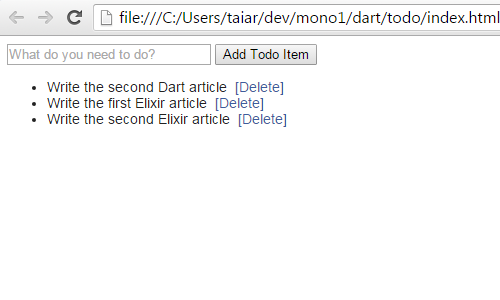
\includegraphics[width=\textwidth]{todo_app.png}
  \caption{Aplicação to-do rodando no browser}
  \label{Rotulo}
\end{figure}

Now I will talk about the usage of the Dart language in this small application.

\subsection{Language structure}

From the very basics, Dart is a class-based, single-inheritance, object-oriented
language with C-style syntax.

The Dart language is also dynamically typed. You can write programs that have no
type annotations whatsoever, and run them, much as you would in JavaScript. One
of the Dart programming language’s most innovative features is the use of
optional types. You may use type annotations in Dart. It will have some
improvements to your program like documentation for humans, documentation for
machines, early error detection (Dart provides a static checker that can warn
you about  potential problems) and sometimes, types can help improve performance
when  compiling to JavaScript.

The static checker acts a lot like in C. It warns you about potential  problems
at compile-time. Many of these warnings are related to types. The static checker
does not produce errors - you can always compile and run your code, no matter
what the checker says.

Let's check out the example:

\begin{lstlisting}[label=dpoint,caption=Dart Warning Example]
class Point {
  final num x, y;
  Point(this.x, this.y);
  Point operator +(Point other) {
    return new Point(x + other.x, y + other.y);
  }

  String toString() {
    return "x: $x, y: $y";
  }
}

main() {
  Point p1 = new Point(0, 0);
  Point p2 = new Point(10, 10);

  int n = p1 + p2;

  print(n);
}
\end{lstlisting}

The code above sends a warning in $int n = p1 + p2;$ saying  $A value of
type 'Point' cannot be assigned to a variable of type 'int'$ if we run the
program with the $checked mode$ turned on. However, the program works nice with
no checking at all.

When no types are provided, Dart avoid complaints by adding a default type
called $dynamic$. We can use this type explicitly:

\begin{lstlisting}[label=dartMap,caption=Dart dynamic type]
Map<String, dynamic> m = {
    'one': new Partridge(),
    'two': new TurtleDove(),
    /* ..., */
    'twelve': new Drummer()};
\end{lstlisting}

Dart has generics too. We can have this kind of list:

\begin{verbatim}
new List<String>();
\end{verbatim}

but you will still be able to write something like

\begin{verbatim}
new List();
\end{verbatim}

and use as a list of $Strings$. The previous example is just a shorthand for

\begin{verbatim}
new List<dynamic>();
\end{verbatim}

The Dart constructor is a method of the class with the same name of the class.
As said before, the protected methods starts with underscore and are not visible
outside the package of the class.

\subsection{Libraries again}

Just like we saw in the language introduction, our program uses external
libraries. The first one is the $dart:html$
library \cite{4_3}. This library manages HTML
elements and other resources for web-based applications that need to interact
with the browser and the DOM (Document Object Model). It includes DOM element
types, CSS styling, local storage, media, speech, events, and more.

The second one is the $dart:indexed_db$
library \cite{4_4}. The IndexedDB is a web
standard for an indexed database which works in the browser. By storing data on
the client in an IndexedDB, a web app gets some advantages, such as faster
performance and persistence. Many browsers supports the use of
IndexedDB \cite{4_5}.In our example, we a using
this database to store the TODO tasks.

The third and last one is the $dart:async$
library \cite{4_6} we saw in the early
examples. In this program, we use $async$ to deal with the events of send
and get data from the HTML5 database (IndexedDB).

In our example, none of these libraries is external to the Dart SDK. So we don't
need to install them with the $pub get$ command. They are all included with a
Dart default installation.

\subsection{Integration with modern browsers (HTML5, IndedexDB and JavaScript API)}

As a language that aims to replace JavaScript on the next years, Dart must have
a strong interoperability with HTML5 elements, browsers functionalities and the
JavaScript existent libraries and apis. Filling the gaps of JavaScript in terms
of functionality is a strategy aligned with Dart purpose to make web app
development more pragmatic.

All of the HTML5 compatibility is implemented in the $dart:html$ library. The
first use of this library we can see in our example is with the function
$querySelector$. This function is like a static method of the library. It finds
the first descendant element of the HTMl document that matches the specified
group of selectors (as parameters of the function) and returns an $Element$
object (that describes a HTML object). The selectors are written in the
form of CSS Selectors \cite{4_7}. JavaScript don't
have a native function to match HTML elements by CSS selectors. This kind of
\"feature missing\" in the JavaScript language brings lots of popularity for some
JavaScript frameworks that aims to fill this kind of gaps in the language. The
most famous of them is jQuery \cite{4_8}
which is so present in JavaScript projects that sometimes is jumbled with the
language itself.

The $Element$ type in Dart \cite{4_9} is an
abstract class, which all HTML elements extend. It implements all HTML browser
behaviors like $events$ as we can see in the snippet:

\begin{verbatim}
querySelector('input#submit').onClick.listen((e) => _onAddTodo());  
\end{verbatim}

The querySelector method matches a Input button Element field with the a ID
attribute equals to \"submit\" and binds to it an event called $onclick$. When
this button is clicked, the private method $_onAddTodo$ is called.

The same patch would be written in vanilla JavaScript in this way:

\begin{lstlisting}[label=jset,caption=Vanilla JavaScript translation]
document.getElementById("submit")
  .addEventListener("click", function(e){
    return _onAddTodo();
  }, false);
\end{lstlisting}

Or even in JavaScript with jQuery this way:

\begin{lstlisting}[label=jjqt,caption=JavaScript with jQuery translation]
$("input#submit").on("click", function(e){
  return _onAddTodo();
});
\end{lstlisting}

The very next browser feature controlled by Dart in the example is the
IndexedDB \cite{4_10} interaction. The Indexed
Database API, or IndexedDB (formerly  WebSimpleDB), is a recommended web browser
standard interface for a local database of records holding simple values and
hierarchical objects. IndexedDB was initially proposed by Oracle in 2009.

The code of the program that open the IndexedDB and return the results is:

\begin{lstlisting}[label=dffexp,caption=Dart open's IndexedDB and return results]
Future open() {
  return window
    .indexedDB
    .open(_TODOS_DB, version: _version, onUpgradeNeeded: _onUpgradeNeeded)
    .then(_onDbOpened)
    .catchError(_onError);
}
\end{lstlisting}

It gets the window of the browser, open the database used by the application,
sets the callback function for when the database is opened and ready to use and
even sets a callback function to deal with errors, all in that lines.

The method that add things on the database is this one:

\begin{lstlisting}[label=dpoint,caption=Dart stores stuff]
Future _addTodo(String text) {
  var trans = _db.transaction(_TODOS_STORE, 'readwrite');
  var store = trans.objectStore(_TODOS_STORE);
  return store.put({
    'text': text,
    'timeStamp': new DateTime.now().millisecondsSinceEpoch.toString()
  }).then((_) => _getAllTodoItems())
  .catchError((e) => _onError);
}
\end{lstlisting}

It opens a transaction \cite{4_11} with the
database, create a object used to store things there and use its method called
put passing the JSON object representing the TODO task to it. Same as before,
the put method is chained with the methods that declares the callbacks for the
function: one for the success and another one for errors.

\subsection{Asynchronous again}

Surely one of the keys concepts to write just about any Dart program is to
understand the asynchronous model as well as the
Future \cite{4_12} and
Stream \cite{4_13} objects.

Very used in our example, a Future is used to represent a potential value, or
error, that will be available at some time in the future. Receivers of a Future
can register callbacks that handle the value or error once it is available.
Those are the callbacks functions I said on the two methods in our previous
topic. A interesting thing is that it applies to the methods that deals with
Input and Output in the program, always heavy operations in any programming
platform.